%\VignetteIndexEntry{Visualize and RNA-seq data normalization with the "NVT" package}
%\VignettePackage{NVT}
%\VignetteEngine{knitr::knitr}

% To compile this document
% library('knitr'); rm(list=ls()); knit('NVT.Rnw')

\documentclass[11pt]{article}\usepackage[]{graphicx}\usepackage[usenames,dvipsnames]{color}
%% maxwidth is the original width if it is less than linewidth
%% otherwise use linewidth (to make sure the graphics do not exceed the margin)
\makeatletter
\def\maxwidth{ %
  \ifdim\Gin@nat@width>\linewidth
    \linewidth
  \else
    \Gin@nat@width
  \fi
}
\makeatother

\definecolor{fgcolor}{rgb}{0.345, 0.345, 0.345}
\newcommand{\hlnum}[1]{\textcolor[rgb]{0.686,0.059,0.569}{#1}}%
\newcommand{\hlstr}[1]{\textcolor[rgb]{0.192,0.494,0.8}{#1}}%
\newcommand{\hlcom}[1]{\textcolor[rgb]{0.678,0.584,0.686}{\textit{#1}}}%
\newcommand{\hlopt}[1]{\textcolor[rgb]{0,0,0}{#1}}%
\newcommand{\hlstd}[1]{\textcolor[rgb]{0.345,0.345,0.345}{#1}}%
\newcommand{\hlkwa}[1]{\textcolor[rgb]{0.161,0.373,0.58}{\textbf{#1}}}%
\newcommand{\hlkwb}[1]{\textcolor[rgb]{0.69,0.353,0.396}{#1}}%
\newcommand{\hlkwc}[1]{\textcolor[rgb]{0.333,0.667,0.333}{#1}}%
\newcommand{\hlkwd}[1]{\textcolor[rgb]{0.737,0.353,0.396}{\textbf{#1}}}%

\usepackage{framed}
\makeatletter
\newenvironment{kframe}{%
 \def\at@end@of@kframe{}%
 \ifinner\ifhmode%
  \def\at@end@of@kframe{\end{minipage}}%
  \begin{minipage}{\columnwidth}%
 \fi\fi%
 \def\FrameCommand##1{\hskip\@totalleftmargin \hskip-\fboxsep
 \colorbox{shadecolor}{##1}\hskip-\fboxsep
     % There is no \\@totalrightmargin, so:
     \hskip-\linewidth \hskip-\@totalleftmargin \hskip\columnwidth}%
 \MakeFramed {\advance\hsize-\width
   \@totalleftmargin\z@ \linewidth\hsize
   \@setminipage}}%
 {\par\unskip\endMakeFramed%
 \at@end@of@kframe}
\makeatother

\definecolor{shadecolor}{rgb}{.97, .97, .97}
\definecolor{messagecolor}{rgb}{0, 0, 0}
\definecolor{warningcolor}{rgb}{1, 0, 1}
\definecolor{errorcolor}{rgb}{1, 0, 0}
\newenvironment{knitrout}{}{} % an empty environment to be redefined in TeX

\usepackage{alltt}

\newcommand{\nvt}{\textit{NVT}}
\newcommand{\lowtilde}{\raise.17ex\hbox{$\scriptstyle\mathtt{\sim}$}}



\RequirePackage{/home/eder/R/x86_64-pc-linux-gnu-library/3.2/BiocStyle/resources/tex/Bioconductor}

\AtBeginDocument{\bibliographystyle{/home/eder/R/x86_64-pc-linux-gnu-library/3.2/BiocStyle/resources/tex/unsrturl}}


\author{Thomas Eder$^{1,2}$, Florian Grebien$^{1}$, Thomas Rattei$^{2}$\\[1em]
  \small{$^{1}$ Ludwig Boltzmann Institute for Cancer Research,} \\
  \small{W{\"a}hringer Stra{\ss}e 13A, 1090 Vienna, Austria.} \\
  \small{$^{2}$ CUBE Division of Computational Systems Biology,} \\
  \small{Department of Microbiology and Ecosystem Science,} \\
  \small{University of Vienna, Althanstra{\ss}e 14, 1090 Vienna, Austria.} }

\title{Visualization and assessment of RNA-Seq data normalization - the Normalization Visualization Tool}
\IfFileExists{upquote.sty}{\usepackage{upquote}}{}
\begin{document}

\maketitle

\begin{abstract}

Measuring differential gene expression is a common task in the analysis of RNA-Seq data.
To identify differentially expressed genes between two samples, it is crucial to normalize the datasets.
While multiple normalization methods are available, all of them are based on certain assumptions that
may or may not be suitable for the type of data they are applied on. Researchers therefore need to select
an adequate normalization strategy for each RNA-Seq experiment. This selection includes exploration of
different normalization methods as well as their comparison. Methods that agree with each other most
likely represent realistic assumptions under the particular experimental conditions.
We developed the \nvt{} package, which provides a fast and simple way to analyze and evaluate
multiple normalization methods via visualization and representation of correlation values, based on a user-defined set of uniformly expressed genes. This vignette explains the use of the package and demonstrates a typical work flow.

  \vspace{1em}

  \textbf{NVT version:} 1.0

  \vspace{1em}

  \begin{center}
    \begin{tabular}{ | l | }
      \hline
      If you use \nvt{} in published research, please cite:  \\
      \\
      T. Eder, F. Grebien, T. Rattei: \textbf{NVT: a fast and simple tool for} \\
      \textbf{the assessment of RNA-Seq normalization strategies}. \\
      \emph{JournalXXX} 2016, \textbf{XX}:XXX. \\
      \url{http://dx.doi.org/xxx/xxx}  \\
      \hline
    \end{tabular}
  \end{center}

\end{abstract}

\newpage

\tableofcontents

\newpage

\section{Installation}

The latest NVT package can be downloaded from: \url{https://github.com/Edert/NVT/releases}. The installation of the package can be done directly in R.

\begin{knitrout}
\definecolor{shadecolor}{rgb}{0.969, 0.969, 0.969}\color{fgcolor}\begin{kframe}
\begin{alltt}
\hlkwd{install.packages}\hlstd{(}\hlkwd{file.path}\hlstd{(}\hlstr{"/home/user/Downloads/"}\hlstd{,}\hlstr{"NVT_1.0.tar.gz"}\hlstd{),}
\hlkwc{repos}\hlstd{=}\hlkwa{NULL}\hlstd{,} \hlkwc{type}\hlstd{=}\hlstr{"source"}\hlstd{)}
\end{alltt}
\end{kframe}
\end{knitrout}

\section{Standard work flow}

Initially the library has to be loaded, which provides access to the data examples \ref{sec:loaddata} and the \nvt functions.

\begin{knitrout}
\definecolor{shadecolor}{rgb}{0.969, 0.969, 0.969}\color{fgcolor}\begin{kframe}
\begin{alltt}
\hlkwd{library}\hlstd{(}\hlstr{"NVT"}\hlstd{)}
\end{alltt}
\end{kframe}
\end{knitrout}

\subsection{Load data}

For the demonstration of the \nvt functions we need gene expression data, so we load the example data provided with the package. We use the two human expression data sets \textit{GSM1275862} and \textit{GSM1275863} from the \href{https://bioconductor.org/packages/release/data/experiment/html/airway.html}{airway}\cite{himes2014} package.

\subsubsection{Load expression data} \label{sec:loaddata}

We simply load the provided data sets \textit{myexp1} from \textit{GSM1275862}, \textit{myexp2} from \textit{GSM1275863} and the length data per gene as \textit{mylen}.

\begin{knitrout}
\definecolor{shadecolor}{rgb}{0.969, 0.969, 0.969}\color{fgcolor}\begin{kframe}
\begin{alltt}
\hlkwd{data}\hlstd{(mylen)}
\hlkwd{data}\hlstd{(myexp1)}
\hlkwd{data}\hlstd{(myexp2)}

\hlcom{#show just the first four elements of the loaded data}
\hlkwd{head}\hlstd{(mylen,}\hlnum{4}\hlstd{)}
\end{alltt}
\begin{verbatim}
##                 Length
## ENSG00000000003   3688
## ENSG00000000005   1881
## ENSG00000000419   4032
## ENSG00000000457  10784
\end{verbatim}
\begin{alltt}
\hlkwd{head}\hlstd{(myexp1,}\hlnum{4}\hlstd{)}
\end{alltt}
\begin{verbatim}
##                 GSM1275862
## ENSG00000000003        679
## ENSG00000000005          0
## ENSG00000000419        467
## ENSG00000000457        260
\end{verbatim}
\end{kframe}
\end{knitrout}

In order to evaluate the expression between the two RNA-seq expression samples, we have to define a list of human housekeeping genes \textit{GAPDH, ALB, ACTB, QARS, HPRT1, ADA} and \textit{POLR2L}.

\begin{knitrout}
\definecolor{shadecolor}{rgb}{0.969, 0.969, 0.969}\color{fgcolor}\begin{kframe}
\begin{alltt}
\hlstd{mylist1}\hlkwb{<-}\hlkwd{c}\hlstd{(}\hlstr{"ENSG00000111640"}\hlstd{,}\hlstr{"ENSG00000163631"}\hlstd{,}\hlstr{"ENSG00000075624"}\hlstd{,}
           \hlstr{"ENSG00000172053"}\hlstd{,}\hlstr{"ENSG00000165704"}\hlstd{,}\hlstr{"ENSG00000196839"}\hlstd{,}
           \hlstr{"ENSG00000177700"}\hlstd{)}
\end{alltt}
\end{kframe}
\end{knitrout}

\subsubsection{Load gene length data}

Instead of using the length data generated directly in R or using a simple flat file, it is also possible to load the gene or exon length data directly from an annotation file in gtf or gff format. This function utilizes the \href{https://bioconductor.org/packages/release/bioc/html/GenomicRanges.html}{GenomicRanges}\cite{lawrence2013} and \href{https://www.bioconductor.org/packages/3.3/bioc/html/rtracklayer.html}{rtracklayer}\cite{lawrence2009} packages.

\begin{itemize}
 \item gff-version: version of the provided gff file $[ gff1,gff2,gff3,gtf ]$
 \item gff-feature: feature to use $[ default: exon ]$
 \item gff-name: name to use $[ default: gene\_id ]$
\end{itemize}

\begin{knitrout}
\definecolor{shadecolor}{rgb}{0.969, 0.969, 0.969}\color{fgcolor}\begin{kframe}
\begin{alltt}
\hlcom{#this line gets the path to the gff file provided in the NVT package}
\hlcom{#(annotation from Chlamydia trachomatis, ACCESSION: NC_000117 )}
\hlstd{mygffpath} \hlkwb{<-} \hlkwd{system.file}\hlstd{(}\hlstr{"extdata"}\hlstd{,} \hlstr{"Ctr-D-UW3CX.gff"}\hlstd{,} \hlkwc{package} \hlstd{=} \hlstr{"NVT"}\hlstd{)}

\hlcom{#this function loads the gff file from the gffpath}
\hlstd{mylen1} \hlkwb{<-} \hlkwd{NVTloadgff}\hlstd{(mygffpath,}\hlstr{"gff3"}\hlstd{,}\hlstr{"gene"}\hlstd{,}\hlstr{"locus_tag"}\hlstd{)}

\hlkwd{head}\hlstd{(mylen1)}
\end{alltt}
\begin{verbatim}
##       Length
## CT001    273
## CT002    303
## CT003   1476
## CT004   1467
## CT005   1092
## CT006    570
\end{verbatim}
\end{kframe}
\end{knitrout}

\subsection{Generate NVTdata objects}

In the first step you need to generate an \textit{NVTdata} object with the \textit{NVTinit} function. Here you have to provide the list of housekeeping genes, the two gene expression samples and the normalization method. Optionally you can also add the gene or exon length data.

The normalization methods are:
\begin{itemize}
 \item N = No normalization
 \item TC = Total count normalization
 \item Med = Median normalization
 \item TMM = Trimmed Mean of M-values normalization
 \item UQ = Upper Quartile normalization
 \item UQ2 = Upper Quartile normalization (from \href{https://www.bioconductor.org/packages/release/bioc/html/NOISeq.html}{NOISeq}\cite{tarazona2011})
 \item Q = Quantile normalization implemented in \href{https://bioconductor.org/packages/release/bioc/html/limma.html}{limma}\cite{ritchie2015}
 \item RPKM = Reads Per Kilobase per Million mapped reads normalization
 \item RPM = Reads Per Million mapped reads normalization
 \item TPM = Transcripts Per Million normalization
 \item DEQ = Relative log expression method included in the \href{https://www.bioconductor.org/packages/release/bioc/html/DESeq.html}{DESeq}\cite{anders2010} package
 \item G = Use the provided genes to normalize
\end{itemize}

For the most methods no length information is required.

\begin{knitrout}
\definecolor{shadecolor}{rgb}{0.969, 0.969, 0.969}\color{fgcolor}\begin{kframe}
\begin{alltt}
\hlstd{mynvt} \hlkwb{<-} \hlkwd{NVTinit}\hlstd{(mylist1,myexp1,myexp2,}\hlstr{"TMM"}\hlstd{)}
\end{alltt}
\end{kframe}
\end{knitrout}

But for RPKM and TPM normalization the length data has to be provided.

\begin{knitrout}
\definecolor{shadecolor}{rgb}{0.969, 0.969, 0.969}\color{fgcolor}\begin{kframe}
\begin{alltt}
\hlstd{mynvt} \hlkwb{<-} \hlkwd{NVTinit}\hlstd{(mylist1,myexp1,myexp2,}\hlstr{"RPKM"}\hlstd{,mylen)}
\end{alltt}
\end{kframe}
\end{knitrout}

\subsubsection{Normalize the NVTdata }

The now initialized \textit{NVTdata} object can be normalized in the next step.

\begin{knitrout}
\definecolor{shadecolor}{rgb}{0.969, 0.969, 0.969}\color{fgcolor}\begin{kframe}
\begin{alltt}
\hlstd{mynorm} \hlkwb{<-} \hlkwd{NVTnormalize}\hlstd{(mynvt)}
\end{alltt}
\begin{verbatim}
## [1] "RPKM normalization!"
\end{verbatim}
\end{kframe}
\end{knitrout}

If required the now normalized data can be retrieved easily.

\begin{knitrout}
\definecolor{shadecolor}{rgb}{0.969, 0.969, 0.969}\color{fgcolor}\begin{kframe}
\begin{alltt}
\hlstd{mynvalues} \hlkwb{<-} \hlkwd{show}\hlstd{(mynorm)}

\hlkwd{head}\hlstd{(mynvalues)}
\end{alltt}
\begin{verbatim}
##                 GSM1275862 GSM1275863
## ENSG00000000003  8.9209656  5.8859979
## ENSG00000000005  0.0000000  0.0000000
## ENSG00000000419  5.6121512  6.1889890
## ENSG00000000457  1.1682249  0.9480595
## ENSG00000000460  0.2395964  0.2196300
## ENSG00000000938  0.0000000  0.0000000
\end{verbatim}
\end{kframe}
\end{knitrout}

\subsection{Visualize expression data}

One of the key features of \nvt is the plotting of the XY-Scatter-Plots and MA-Plots. This can be done with the functions:
\textit{NVTplot}, \textit{NVTadvancedplot}, \textit{NVTmaplot} and \textit{NVTadvancedmaplot}.

\newpage

\subsubsection{Simple plot functions}

The normalized \textit{NVTdata} object can be visualized with the plot function. With the second parameter you can modify the size-ratio of the text and the data points. All expression values are shown as grey dots and the linear model as red line, it is calculated with the data from the housekeeping genes only. The dashed grey line highlights the diagonal, so the perfect correlation between the two data sets.

\begin{knitrout}
\definecolor{shadecolor}{rgb}{0.969, 0.969, 0.969}\color{fgcolor}\begin{kframe}
\begin{alltt}
\hlkwd{NVTplot}\hlstd{(mynorm,}\hlnum{0.4}\hlstd{)}
\end{alltt}
\end{kframe}
\end{knitrout}

\begin{figure}[!h]
\centering
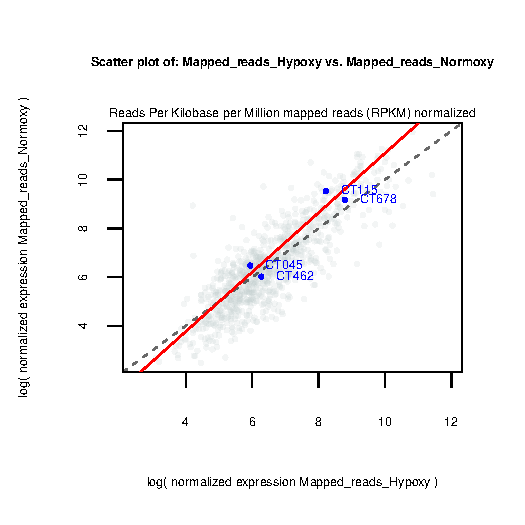
\includegraphics[width=.8\textwidth]{figure/simpleplot-1}
\caption{
  \textbf{XY-Scatter-Plot.}
  The resulting plot from the simple NVTplot function}
\label{fig:XY}
\end{figure}

\newpage

The \textit{NVTplotma} function works similar but produces an MA-Plot instead of a Scatter-Plot.

\begin{knitrout}
\definecolor{shadecolor}{rgb}{0.969, 0.969, 0.969}\color{fgcolor}\begin{kframe}
\begin{alltt}
\hlkwd{NVTmaplot}\hlstd{(mynorm,}\hlnum{0.4}\hlstd{)}
\end{alltt}
\end{kframe}
\end{knitrout}

\begin{figure}[!h]
\centering
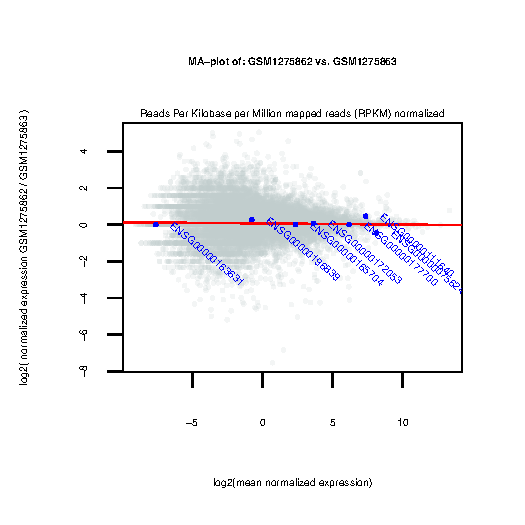
\includegraphics[width=.8\textwidth]{figure/simplemaplot-1}
\caption{
  \textbf{MA-Plot.}
  The resulting plot from the simple NVTmaplot function}
\label{fig:MA}
\end{figure}

\newpage

\subsubsection{Advanced plot functions}

The \textit{NVTadvancedplot} plots via \href{https://cran.r-project.org/web/packages/ggplot2/index.html}{ggplot2}\cite{wickham2009} and the size parameters control data points, text and labels separately. Here we use the default values of 1 for the data points and the text and increase the labels of the housekeeping genes to 2. Again the grey dots represent the expression data and their density is visualized by the rug in dark red for x- and y-axis.
The linear model of the housekeeping gene data is shown in red and the diagonal is highlighted as grey dashed line. As we want to compare different methods we now normalize with the TMM method.

\begin{knitrout}
\definecolor{shadecolor}{rgb}{0.969, 0.969, 0.969}\color{fgcolor}\begin{kframe}
\begin{alltt}
\hlstd{mynvt} \hlkwb{<-} \hlkwd{NVTinit}\hlstd{(mylist1,myexp1,myexp2,}\hlstr{"TMM"}\hlstd{,mylen)}
\hlstd{mynorm} \hlkwb{<-} \hlkwd{NVTnormalize}\hlstd{(mynvt)}
\end{alltt}
\begin{verbatim}
## [1] "Trimmed Mean of M-values normalization!"
\end{verbatim}
\begin{alltt}
\hlkwd{NVTadvancedplot}\hlstd{(mynorm,}\hlnum{1}\hlstd{,}\hlnum{1}\hlstd{,}\hlnum{1}\hlstd{)}
\end{alltt}
\end{kframe}
\end{knitrout}

\begin{figure}[!h]
\centering
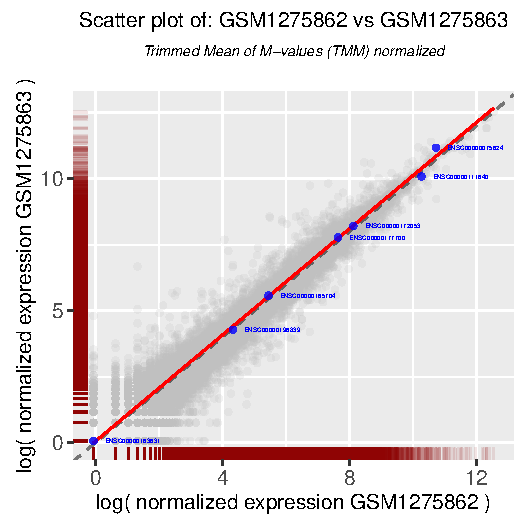
\includegraphics[width=.8\textwidth]{figure/advancedplot-1}
\caption{
  \textbf{Advanced XY-Scatter-Plot.}
  The NVTadvancedplot function results in a plot produced by ggplot2 with a rug on both axis, indicating the density of the data-points}
\label{fig:adXY}
\end{figure}

\newpage

As alternative there is also the possiblity to create an MA-Plot with the \textit{NVTadvancedmaplot} function.

\begin{knitrout}
\definecolor{shadecolor}{rgb}{0.969, 0.969, 0.969}\color{fgcolor}\begin{kframe}
\begin{alltt}
\hlkwd{NVTadvancedmaplot}\hlstd{(mynorm,}\hlnum{1}\hlstd{,}\hlnum{1}\hlstd{,}\hlnum{1}\hlstd{)}
\end{alltt}
\end{kframe}
\end{knitrout}

\begin{figure}[!h]
\centering
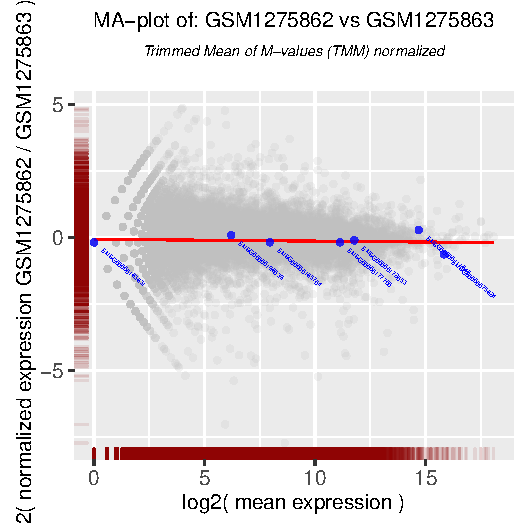
\includegraphics[width=.8\textwidth]{figure/advancedmaplot-1}
\caption{
  \textbf{Advanced MA-Plot.}
  The NVTadvancedmaplot function results in a plot produced by ggplot2 with a rug on both axis, indicating the density of the data-points}
\label{fig:adMA}
\end{figure}

\newpage

\subsubsection{Linear model}

If required, the linear model plotted as red line can be retrieved with the \textit{NVTlm} function.

\begin{knitrout}
\definecolor{shadecolor}{rgb}{0.969, 0.969, 0.969}\color{fgcolor}\begin{kframe}
\begin{alltt}
\hlstd{mylm} \hlkwb{<-} \hlkwd{NVTlm}\hlstd{(mynorm)}

\hlkwd{summary}\hlstd{(mylm)}
\end{alltt}
\begin{verbatim}
## 
## Call:
## lm(formula = sample2 ~ sample1)
## 
## Residuals:
## ENSG00000111640 ENSG00000163631 ENSG00000075624 ENSG00000172053 ENSG00000165704 
##        -0.30369         0.07392         0.32555        -0.02492         0.03966 
## ENSG00000196839 ENSG00000177700 
##        -0.13993         0.02941 
## 
## Coefficients:
##             Estimate Std. Error t value Pr(>|t|)    
## (Intercept)  0.05662    0.17320   0.327    0.757    
## sample1      1.00548    0.02310  43.522 1.21e-07 ***
## ---
## Signif. codes:  0 '***' 0.001 '**' 0.01 '*' 0.05 '.' 0.1 ' ' 1
## 
## Residual standard error: 0.2128 on 5 degrees of freedom
## Multiple R-squared:  0.9974,	Adjusted R-squared:  0.9968 
## F-statistic:  1894 on 1 and 5 DF,  p-value: 1.209e-07
\end{verbatim}
\end{kframe}
\end{knitrout}

\subsection{Correlation values}

In addition to the graphical representation of the gene expression data, the correlation coefficients of the housekeeping genes of the two samples can be calculated with the functions \textit{NVTpearson}, \textit{NVTrmsd} and \textit{NVTmae}.

\subsubsection{Pearson correlation}

The Pearson correlation coefficient of the normalized expression of the housekeeping genes is calculated with the following command, using an already normalized \textit{NVTdata} object.

\begin{knitrout}
\definecolor{shadecolor}{rgb}{0.969, 0.969, 0.969}\color{fgcolor}\begin{kframe}
\begin{alltt}
\hlkwd{NVTpearson}\hlstd{(mynorm)}
\end{alltt}
\begin{verbatim}
##     pearson     p-value 
## 0.962199426 0.000522815
\end{verbatim}
\end{kframe}
\end{knitrout}

\subsubsection{RMSD and MEA correlation}

The root mean square error (RMSE) also called the root mean square deviation (RMSD) is calculated with the \textit{NVTrmsd} function.

\begin{knitrout}
\definecolor{shadecolor}{rgb}{0.969, 0.969, 0.969}\color{fgcolor}\begin{kframe}
\begin{alltt}
\hlkwd{NVTrmsd}\hlstd{(mynorm)}
\end{alltt}
\begin{verbatim}
##     RMSD 
## 9725.145
\end{verbatim}
\end{kframe}
\end{knitrout}

And the mean absolute error (MAE) can be calculated and retrieved with the \textit{NVTmae} function.

\begin{knitrout}
\definecolor{shadecolor}{rgb}{0.969, 0.969, 0.969}\color{fgcolor}\begin{kframe}
\begin{alltt}
\hlkwd{NVTmae}\hlstd{(mynorm)}
\end{alltt}
\begin{verbatim}
##      MAE 
## 4405.926
\end{verbatim}
\end{kframe}
\end{knitrout}

\subsection{Test all methods}

To test more normalization methods on the provided data sets in one single step, the correlation coefficients of all implemented normalization methods can be calculated with the \textit{NVTtestall} function.
It requires a normalized \textit{NVTdata} object and the correlation coefficient you are interested in. The method can be defined with:

\begin{itemize}
 \item p = Pearson correlation
 \item rmsd = root mean square deviation
 \item mae = mean absolute error
\end{itemize}

\begin{knitrout}
\definecolor{shadecolor}{rgb}{0.969, 0.969, 0.969}\color{fgcolor}\begin{kframe}
\begin{alltt}
\hlkwd{NVTtestall}\hlstd{(mynorm,}\hlstr{"p"}\hlstd{)}
\end{alltt}
\begin{verbatim}
## [1] "No normalization!"
## [1] "Total count normalization!"
## [1] "Median normalization!"
## [1] "Trimmed Mean of M-values normalization!"
## [1] "Upper Quartile normalization!"
## [1] "Upper Quartile normalization (from NOISeq)!"
## [1] "Quantile normalization!"
## [1] "RPKM normalization!"
## [1] "RPM normalization!"
## [1] "DESeq normalization!"
## [1] "Using DESeq"
## [1] "Input counts are not integer, converting them!"
## [1] "TPM normalization!"
## [1] "Normalization by given gene-set!"
## [1] "ENSG00000111640" "ENSG00000163631" "ENSG00000075624" "ENSG00000172053"
## [5] "ENSG00000165704" "ENSG00000196839" "ENSG00000177700"
##        pearson      p-value
## Q    0.9706297 0.0002794844
## DEQ  0.9621994 0.0005228150
## G    0.9621994 0.0005228150
## N    0.9621994 0.0005228150
## Med  0.9621994 0.0005228150
## UQ2  0.9621994 0.0005228150
## RPM  0.9621994 0.0005228150
## TMM  0.9621994 0.0005228150
## UQ   0.9621994 0.0005228150
## TC   0.9621994 0.0005228150
## RPKM 0.9457678 0.0012774997
## TPM  0.9457678 0.0012774997
\end{verbatim}
\end{kframe}
\end{knitrout}

\section{Session Info}

\begin{itemize}\raggedright
  \item R version 3.2.5 (2016-04-14), \verb|x86_64-pc-linux-gnu|
  \item Locale: \verb|LC_CTYPE=en_US.UTF-8|, \verb|LC_NUMERIC=C|, \verb|LC_TIME=de_AT.UTF-8|, \verb|LC_COLLATE=en_US.UTF-8|, \verb|LC_MONETARY=de_AT.UTF-8|, \verb|LC_MESSAGES=en_US.UTF-8|, \verb|LC_PAPER=de_AT.UTF-8|, \verb|LC_NAME=C|, \verb|LC_ADDRESS=C|, \verb|LC_TELEPHONE=C|, \verb|LC_MEASUREMENT=de_AT.UTF-8|, \verb|LC_IDENTIFICATION=C|
  \item Base packages: base, datasets, graphics, grDevices, methods, stats,
    utils
  \item Other packages: knitr~1.12.3, NVT~1.0
  \item Loaded via a namespace (and not attached): annotate~1.48.0,
    AnnotationDbi~1.32.3, Biobase~2.30.0, BiocGenerics~0.16.1,
    BiocParallel~1.4.3, BiocStyle~1.8.0, Biostrings~2.38.4, bitops~1.0-6,
    colorspace~1.2-6, DBI~0.3.1, DESeq~1.22.1, evaluate~0.8.3, formatR~1.3,
    futile.logger~1.4.1, futile.options~1.0.0, genefilter~1.52.1,
    geneplotter~1.48.0, GenomeInfoDb~1.6.3, GenomicAlignments~1.6.3,
    GenomicRanges~1.22.4, ggplot2~2.1.0, grid~3.2.5, gtable~0.2.0, highr~0.5.1,
    IRanges~2.4.8, labeling~0.3, lambda.r~1.1.7, lattice~0.20-33, limma~3.26.9,
    magrittr~1.5, Matrix~1.2-5, munsell~0.4.3, NOISeq~2.14.1, parallel~3.2.5,
    plyr~1.8.3, RColorBrewer~1.1-2, Rcpp~0.12.4, RCurl~1.95-4.8,
    Rsamtools~1.22.0, RSQLite~1.0.0, rtracklayer~1.30.4, S4Vectors~0.8.11,
    scales~0.4.0, splines~3.2.5, stats4~3.2.5, stringi~1.0-1, stringr~1.0.0,
    SummarizedExperiment~1.0.2, survival~2.39-2, tools~3.2.5, XML~3.98-1.4,
    xtable~1.8-2, XVector~0.10.0, zlibbioc~1.16.0
\end{itemize}




\newpage

\bibliography{library}

\end{document}
